\lstdefinestyle{yaml}{
     basicstyle=\color{red}\footnotesize,
     rulecolor=\color{black},
     string=[s]{'}{'},
     stringstyle=\color{red},
     comment=[l]{:},
     commentstyle=\color{black},
     morecomment=[l]{-}
 }
 \lstset{numbers=left}
 
\chapter{Cloud Infrastructure} \label{ch:AWSUsedServices}
As discussed in previous chapters, the development of \gls{ac:sdv} technology requires a cloud infrastructure to handle server-side operations. \gls{ac:aws} is a leading player in the cloud world, and therefore an ideal alternative for the advancement of \gls{ac:sdv}, as well as an active partner in the implementation of technologies that contribute to the creation of a publicly available \gls{ac:sdv} for all. The following discussion introduces and analyzes, via \gls{ac:aws} documentation the key tools for successful \gls{ac:poc} implementation which will be explored in more detail later.

\section{AWS Used Services}
Among the hundreds of services offered by \gls{ac:aws}, here are the ones that are used to build a cloud infrastructure that is useful for work purposes. The following services have been sorted in order of importance. In particular, services dedicated to development support, services related to \gls{ac:iot} devices, services related to execution, services related to data management, and services related to virtual machine instances are analyzed.
\begin{itemize}
    \item[] \textbf{\gls{ac:awscli}} 
    
    The \gls{ac:awscli} is an essential tool for developing with AWS services. It allows interaction with \gls{ac:aws} services from the command line of a local \gls{ac:pc}, enabling the creation of infrastructure and management of properties from the command line.
    
    \item[] \textbf{AWS Boto} 
    
    \textit{Boto} is an \gls{ac:aws} \gls{ac:sdk} made for \textit{Python}. A \gls{ac:sdk}, more generally, is a set of creation tools specifically for developing and running software in a single platform. It includes resources such as documentation, examples, and APIs to facilitate faster application development. Boto basically works as an interface for applications that need to interact with and take advantage of the services provided by \gls{ac:aws}. The \gls{ac:aws} \gls{ac:sdk} for \textit{JavaScript v3} is another example of an \gls{ac:sdk} for \textit{JavaScript} that works basically in the same way.
    \begin{figure}[h]  % 'h' significa che la figura viene posizionata qui
        \centering
        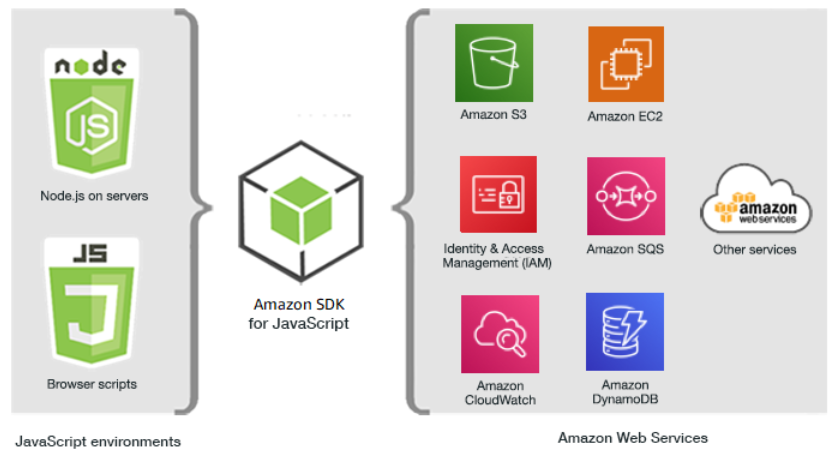
\includegraphics[width=0.8\textwidth]{images/AWSSDK.png}  % Sostituisci 'nome_immagine' con il nome del tuo file immagine e l'estensione
        \caption{The high level rappresentation of the \textit{AWS SDK} for \textit{JavaScript v3} \cite{AWSSDK}}
        \label{fig:AWSSDK}
    \end{figure}
    
    \item[] \textbf{\gls{ac:awscdk}} 
    
    The \gls{ac:awscdk} "is an open-source software development framework for defining cloud infrastructure in code and provisioning it through \textit{AWS CloudFormation}" \cite{WhatIsTheAWSCDK}. It is compatible with both \textit{JavaScript} and \textit{Python} languages and it support the automatic creation of several services with just one execution command. This code-tool was used in the final phase of the \gls{ac:poc} design to automate the creation of the stack comprising all the services used.
    
    \item[] \textbf{AWS IoT Core} 
    
    \textit{AWS IoT Core} provides the ability to connect \gls{ac:iot} devices to \gls{ac:aws} cloud services. \textit{AWS IoT Core} enables the connection of \gls{ac:iot} devices to \gls{ac:aws} cloud services. It simplifies the integration of \gls{ac:iot} devices with other \gls{ac:aws} services. This is especially relevant in the automotive industry, where vehicle system \gls{ac:ecu}s can be viewed as multiple \gls{ac:iot} devices. Communication between the device and \gls{ac:aws} services can occur in several modes, with the \gls{ac:mqtt} protocol being the most important for this project. The device can be connected by developing applications that utilize the \gls{ac:sdk} libraries. Once the data is transmitted, it can be utilized for various purposes such as testing, validation, and analysis. The \gls{ac:aws} \gls{ac:iot} services, including the \textit{AWS IoT Core} service, allow for the creation of digital twins of physical \gls{ac:iot} devices, known as \textit{Thing}, and monitoring of traffic on selected \gls{ac:mqtt} channels. These elements will be explored in greater detail later in the \gls{ac:poc} analysis were it is use as the connection point between the \gls{ac:iot} device an the cloud infrastructure.
    \begin{figure}[h]  % 'h' significa che la figura viene posizionata qui
        \centering
        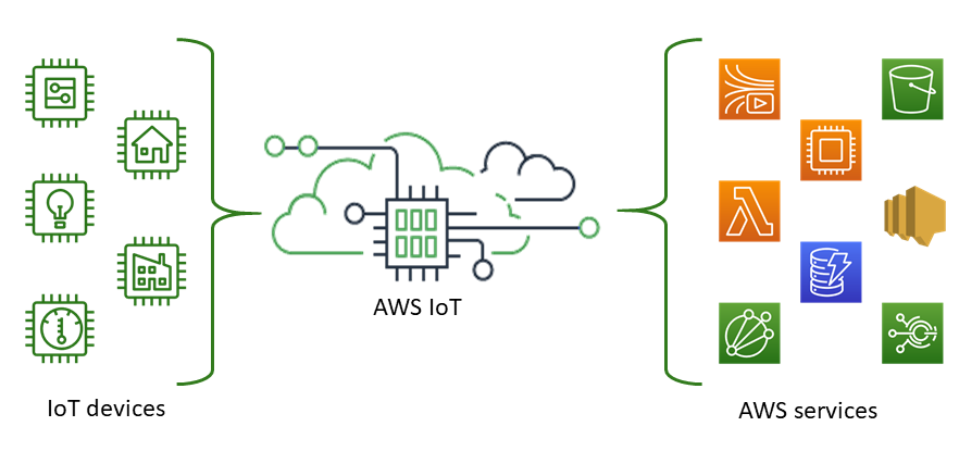
\includegraphics[width=0.8\textwidth]{images/AWSIoTCore.png}  % Sostituisci 'nome_immagine' con il nome del tuo file immagine e l'estensione
        \caption{\textit{AWS IoT Core} connection system between \textit{IoT} device and \textit{AWS} service \cite{AWSIoTCore}}
        \label{fig:AWSIoTCore}
    \end{figure}

    \item[] \textbf{AWS IoT Greengrass}
    
    "\textit{AWS IoT Greengrass} is an open source \gls{ac:iot} edge runtime and cloud service that helps you build, deploy and manage IoT applications on devices" \cite{AWSIoTGreengrass}. It is designed to work with intermittent connections and can manage fleets of devices in the field, locally or remotely, using \gls{ac:mqtt} or other protocols. Once installed, this service can be accessed through the command line. It was utilized in the early stages of project development as an agent to handle updates on the vehicle simulator side. However, this solution will be replaced by a custom solution as explained later.
    
    \item[] \textbf{\gls{ac:awsiam}}
    
    "\gls{ac:awsiam} is a web service for securely controlling access to AWS services [...] such as access keys, and permissions that control which AWS resources users and applications can access" \cite{AWSIAM}. \gls{ac:awsiam} is a service that provides a powerful access management mechanism. However, for the purpose of this thesis, only the relevant functionality to the project will be analyzed, specifically \gls{ac:awsiam}'s role management capabilities.An IAM role is an identity within \gls{ac:aws} that can be assigned specific permissions via permission policies to determine what actions can and cannot be taken. Roles can be assumed by users, applications, or services that do not normally have access to the specific \gls{ac:aws} resources. The \gls{ac:awsiam} service also provides another important concept, that of policy, which is an AWS object that, when attached to an identity (including roles) or a resource, enables the creation of permissions and access control to other resources. For example, as explained below, a policy can be attached to the cloud representation of an \textit{AWS IoT Core} device to enable the connection of the physical dual \gls{ac:iot} device or to grant Subscriber or \textit{Publisher} permissions in a communication via \gls{ac:mqtt} protocol.
    
    \item[] \textbf{AWS Lambda}
    
    \textit{AWS Lambda} is a computing service that provides the ability to run code without servers. It runs code on a high-performance computing infrastructure and handles administrative tasks related to computing resources autonomously, such as server and operating system management, capacity provisioning, automatic scaling, and logging. It is possible to run code for potentially any type of backend application or service \cite{AWSLambda}. Code can be written directly in \textit{Lambda} console or imported from the local environment, and it supports several languages, including \textit{Python} and \textit{JavaScript}. The \textit{Lambda} service can also manipulate data from other \gls{ac:aws} services or manage tasks with services outside \gls{ac:aws} as will be analyzed below.
    
    \item[] \textbf{Amazon Cloudwatch}
    
    \textit{Amazon CloudWatch} is a system to monitor the \gls{ac:aws} resources and the applications running on the infrastructure in real time. With the use of \textit{Amazon CloudWatch} it is possible to collect and track metrics from other \gls{ac:aws} services such as \textit{Lambda}, which are numeric variables that can be measured and analyzed for resources applications \cite{AWSCloudwatch}. Practically this service represents the center for viewing and analyzing logs from the various \gls{ac:aws} services in use.

    \item[] \textbf{AWS CodePipeline}
    
    \textit{AWS CodePipeline} is a fully managed continuous delivery service that automates release pipelines for software updates. It enables fast and reliable updates to applications and infrastructure, facilitating the rapid release of new features, iterative development based on feedback, and bug detection through testing every code change. The software release process can be modeled and configured quickly via the \textit{Stages} execution. A \textit{Stage} is a logical unit that creates an isolated environment and allows for the execution of a limited number of concurrent software changes. Each stage contains actions that are executed on application artifacts, such as source code from \textit{AWS CodeCommit}. For instance, as shown in the image \ref{fig:AWSCodePipeline}, it is feasible to establish a software development pipeline that incorporates a CodeCommit repository as its source stage. This way, a CodeCommit-related event triggers the pipeline execution which then proceeds to the software build stage. An execution is defined as a series of modifications released from a pipeline. Each execution represents a set of modifications, such as a merged commit or a manual release of the last commit. Subsequently, the pipeline moves on to the test stage where the desired tests can be launched via \textit{AWS CodeBuild}, and finally delivers the application for production. 
    \begin{figure}[h]  % 'h' significa che la figura viene posizionata qui
        \centering
        \includegraphics[width=0.8\textwidth]{images/AWSCodePipeline.png}  % Sostituisci 'nome_immagine' con il nome del tuo file immagine e l'estensione
        \caption{An example of a \textit{AWS CodePipeline} in which some stages are reported \cite{AWSCodepipeline}}
        \label{fig:AWSCodePipeline}
    \end{figure}
    
    \item[] \textbf{AWS CodeBuild}
    
    \textit{AWS CodeBuild} is a fully managed build service in the cloud that provides source code compilation, unit testing, and production of executable programs ready for distribution \cite{AWSCodebuild}. \textit{AWS CodeBuild} provides "out-of-the-box" configuration of compilation environments for popular programming languages, such as \textit{Python}. It is also possible to create build platforms for programming languages for which there is no preconfiguration, but in this case it is necessary to leverage multiple \gls{ac:aws} services. It is also possible to use CodeBuild to run tests on application code using for example the \textit{Pytest} tool that allows you to test \textit{Python} code.
    
    \item[] \textbf{AWS CodeCommit}
    
    "\textit{AWS CodeCommit} is a version control service that enables you to privately store and manage \textit{Git} repositories in the \gls{ac:aws} cloud" \cite{AWSCodecommit}. This service becomes particularly interesting in the context of multiple services working together, including \textit{Lambda}, \textit{CodePipeline}, and \textit{CodeBuild}, because it allows the repository's \textit{Git} and all its associated events (such as commit and push) to be used to trigger events that can automate various operations, such as triggering a pipeline in CodePipeline. As a result, \textit{CodePipelines} typically use a \textit{CodeCommit} repository as their input source stage that contains the code necessary for the subsequent stages.
    
    \item[] \textbf{\gls{ac:as3}}
    
    "\gls{ac:as3} is an object storage service that offers industry-leading scalability, data availability, security, and performance" \cite{AWSamazonS3}. The data saved in the storage is physically placed in multiple locations to ensure the durability of the data even if there is tampering with an item due to the presence of these copies; optionally, it can also be chosen to store the data in a single location to reduce the cost of the service. \gls{ac:as3} can be used for data collection, aggregation, and analysis in many contexts and scenarios, but in the scope of this project, this service is used to store data that is transferred from one stage of the \textit{CodePipeline} to another. \textit{AWS CodePipeline} service automatically implements this method of output use. However, data stored in \gls{ac:as3} from one stage to another can be manipulated through integration with other \gls{ac:aws} services, such as \textit{Lambda}. This service is not explicitly mentioned in the description of the project as it plays a secondary role in the implementation, but it is present, even if not always visible to the user.
    \begin{figure}[h]  % 'h' significa che la figura viene posizionata qui
        \centering
        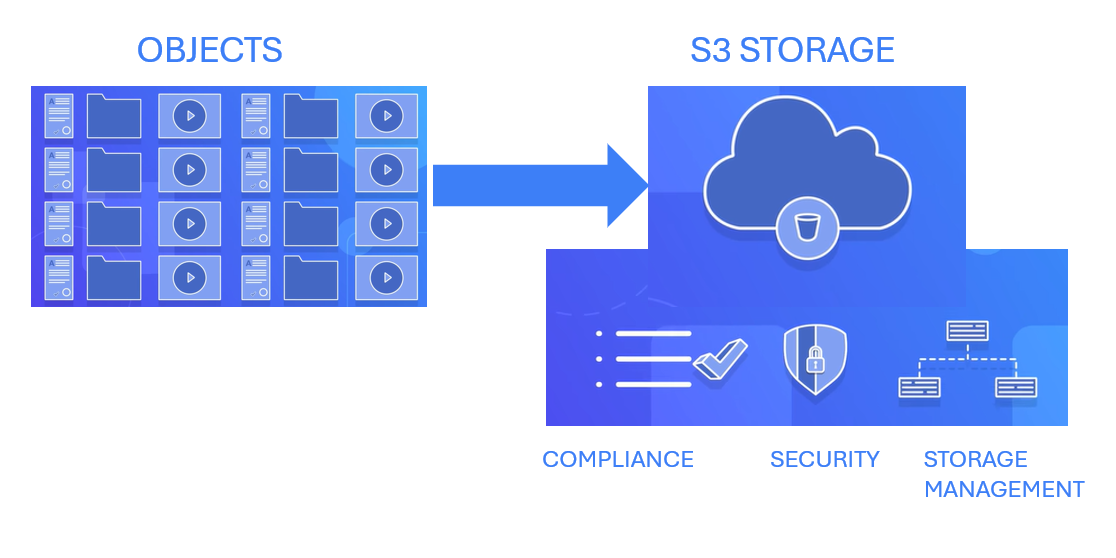
\includegraphics[width=0.8\textwidth]{images/AWSS3.png}  % Sostituisci 'nome_immagine' con il nome del tuo file immagine e l'estensione
        \caption{\textit{Amazon S3} high level storing rappresentation}
        \label{fig:AWSS3}
    \end{figure}

    \item[] \textbf{Amazon Kinesis Data Streams}
    
    \textit{Amazon Kinesis Data Streams} is used to collect and process large streams of data records in real time, and eventually route them through other \gls{ac:aws} services to various data collection and analysis applications, such as \gls{ac:as3} as it is shown in the image \ref{fig:AmazonKinesis}. "The delay between the time a record is put into the stream and the time it can be retrieved (put-to-get delay) is typically less than 1 second. In other words, a \textit{Kinesis Data Streams} application can start consuming the data from the stream almost immediately after the data is added" \cite{AWSKinesis}. The \textit{Kinesis Data Stream} service allows for the selection of specific data based on characteristics through an integrated query system. Additionally, this service can serve as input for \textit{Lambda} functions or to populate databases. 
    \begin{figure}[h]  % 'h' significa che la figura viene posizionata qui
        \centering
        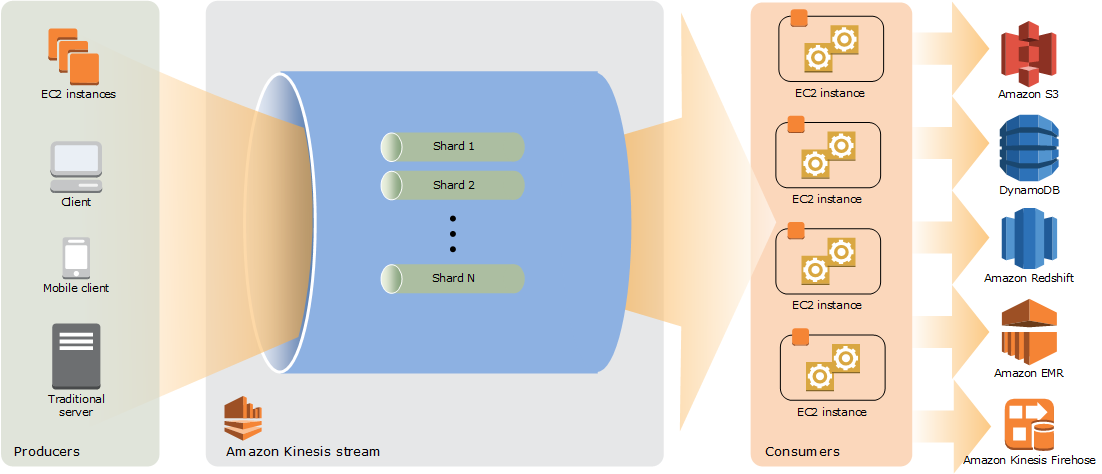
\includegraphics[width=0.8\textwidth]{images/AmazonKinesis.png}  % Sostituisci 'nome_immagine' con il nome del tuo file immagine e l'estensione
        \caption{Illustration of the high-level architecture of \textit{Kinesis Data Streams} with some examples of services that use the output of the stream. \cite{AmazonKinesis}}
        \label{fig:AmazonKinesis}
    \end{figure}
 
    \item[] \textbf{Amazon Timestream}
    
    \textit{Amazon Timestream} is a time-series database that allows you to store and easily analyze large amounts of data stored at regular intervals, ensuring that the time-series data is always encrypted, whether at rest or in transit. This service simplifies the complex process of managing the lifecycle of data by providing storage tiering with an in-memory store for current data and a magnetic store for historical data using \gls{ac:as3} space. The transition of data between these two storage types is enabled through the use of user-configurable policies. The data lifecycle management mechanism makes \textit{Amazon Timestream} ideal for handling telemetry data from \gls{ac:iot} devices, for example. The service also provides a built-in interface for accessing data through a query engine \cite{AWSTimestream}. The \textit{Amazion Timestrem} service also provides an interface for \textit{Grafana} to view and analyze stored data, which will be explored later.
    
    \item[] \textbf{DinamoDB}
    
    \textit{Amazon DynamoDB} is a full-featured NoSQL database service that provides high perfomances both speed and scalability. \textit{Amazon DynamoDB} removes the administrative complexity of running and scaling your distributed database, so there's no need to manage provisioning, hardware setup and configuration, replication, software patching, or cluster sizing. \textit{Amazon DynamoDB} also provides encryption at rest, eliminating the operational costs associated with protecting sensitive data. \textit{Amazon DynamoDB} provides the ability to change the allocation of resources needed to store data in real time to use only the resources required. Additionally, \textit{Amazon DynamoDB} offers on-demand backup functionality for long-term retention and archival purposes, as well as "point-in-time" recovery to safeguard against accidental write or delete operations. This feature enables users to restore a table to any point within the last 35 days \cite{AWSDynamoDB}. Note that this service was not utilized in the final version of the project, but was considered during development as an alternative for data storage and as a case study for understanding the data storage mechanisms used by \gls{ac:aws} services.
    
    \item[] \textbf{AWS System Manager}
    
    \textit{AWS Systems Manager} is a service that provides visibility and control of the infrastructure on \gls{ac:aws}. It allows users to view operational data from multiple \gls{ac:aws} services and manage the automation of operational tasks across different \gls{ac:aws} resources \cite{AWSSM}. The \textit{AWS System Manager} service is particularly relevant to the project due to its application management capability, namely the \textit{Parameter Store}. \textit{Parameter Store} is used to securely store configuration data and secrets, such as passwords, connection strings, and \gls{ac:ami} identifiers. Values are stored hierarchically by assigning hierarchical names to stored values using the "/" character, while maintaining the uniqueness of the name. For example, names such as "Parameters/Parameter1", "Parameters/Parameter2" can be used. In addition, it is possible to choose whether to store the data as plain text or encrypted data. Stored data can be retrieved directly from other services, for example, by interacting with Lambdas and \gls{ac:sdk} code functions.
     
    \item[] \textbf{\gls{ac:aecr}}
    
    "\gls{ac:aecr} is an \gls{ac:aws} managed container image registry service that is secure, scalable, and reliable. \gls{ac:aecr} supports private repositories with resource-based permissions using \gls{ac:awsiam}. This is so that specified users or instances can access [...] container repositories and images" \cite{AmazonECR}. Basically, as shown in the figure \ref{fig:AWSECR}, once the software has been produced and packaged, for example through the use of the \textit{CodeBuild} service, it can be uploaded to \gls{ac:aecr}. The \gls{ac:aecr} takes care of encrypting the image and controlling access to it, and then automatically manages the entire lifecycle of the image. Once the image is on \gls{ac:aecr}, it can be used either as an image for local download or through other \gls{ac:aws} services. 
    \begin{figure}[h]  % 'h' significa che la figura viene posizionata qui
        \centering
        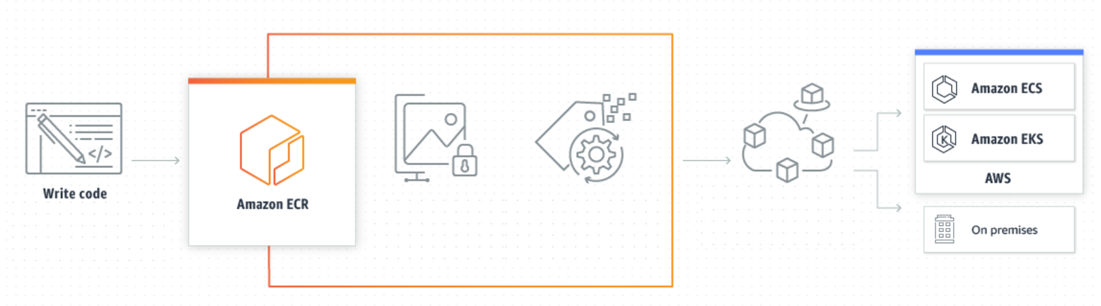
\includegraphics[width=0.8\textwidth]{images/AWSECR.png}  % Sostituisci 'nome_immagine' con il nome del tuo file immagine e l'estensione
        \caption{Example of how \textit{Amazon ECR} works in production and for pulling images \cite{AWSECR}}
        \label{fig:AWSECR}
    \end{figure}
    
    \item[] \textbf{\gls{ac:aec2}}
    
    \gls{ac:aec2} provides scalable, on-demand computing capacity in the \gls{ac:aws} cloud. With \gls{ac:aec2}, users can create and use virtual machines in the cloud, instantiating resources as needed to perform compute operations. \gls{ac:aec2} is a common choice for rapidly deploying applications because it provides an excellent computing resource at a low cost \cite{AWSEC2}, and it is possible to manage networks of different instances of \gls{ac:aec2} virtual machines through \gls{ac:avpc} and set their relative security, either on a per-instance basis or on an overall network basis. Additionally, it is possible to increase the capacity (scale up) of the instance after creation to handle computationally heavy tasks, such as spikes in website traffic. Conversely, if utilization decreases, capacity can be reduced (scale down). \gls{ac:aec2} instances can be launched with \gls{ac:ami}s, which are preconfigured templates containing the necessary components to use the server, including the operating system and additional software. \gls{ac:aws} provides pre-built \gls{ac:ami}s, but it is also possible to create your own \gls{ac:ami}s using containers. Furthermore, it is possible to connect to an \gls{ac:aec2} instance through various communication systems, such as using \gls{ac:ssh} keys provided at the time of instance creation.
          
\end{itemize}

\section{Infrastructure Schema}
All of the previously listed services have been useful, both as an active part in the project's realization and as potential options for the project's implementation, which will be analyzed below. 

After reviewing the various services theoretically, it is now possible to understand a high-level look at how the various services interact with each other.
The interaction system is intricate and consists of two main circuits. The image \ref{fig:AWSDataServices} shows the management of data from the \gls{ac:tcu} edge device in the first part. The data is sent to the cloud via the \textit{IoT Core Thing}, inserted into a \textit{Kinesis} channel, and then sent to a \textit{Timestream} database in relevant tables.
\begin{figure}[h]  % 'h' significa che la figura viene posizionata qui
    \centering
    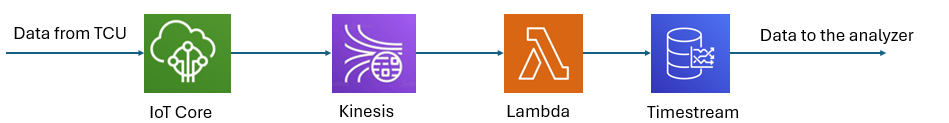
\includegraphics[width=1\textwidth]{images/AWS_data_services.png}  % Sostituisci 'nome_immagine' con il nome del tuo file immagine e l'estensione
    \caption{The high level rappresentation of the \textit{AWS} services for the data managing}
    \label{fig:AWSDataServices}
\end{figure}

\begin{figure}[h]  % 'h' significa che la figura viene posizionata qui
    \centering
    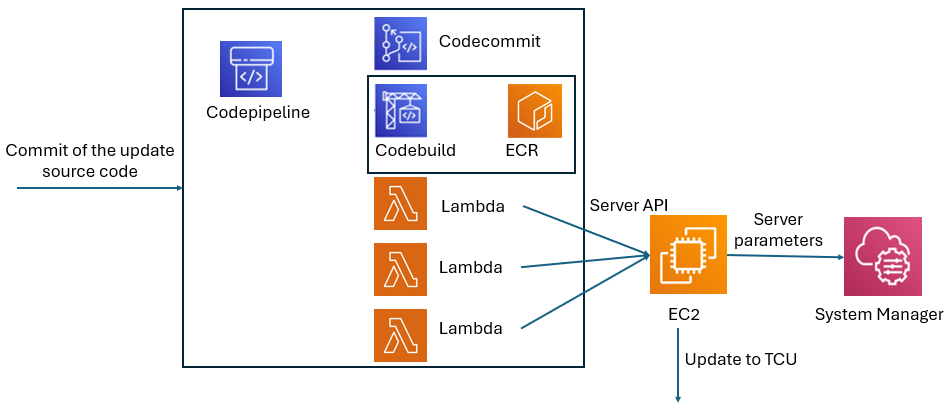
\includegraphics[width=1\textwidth]{images/AWS_update_services.png}  % Sostituisci 'nome_immagine' con il nome del tuo file immagine e l'estensione
    \caption{The high level rappresentation of the \textit{AWS} services for the update managing}
    \label{fig:AWSUpdateServices}
\end{figure}
During the second part of the service interaction shown in the image \ref{fig:AWSUpdateServices}, the system consists of a \textit{CodePipeline} that can be triggered by a \textit{CodeCommit} event acting as a source. The pipeline includes a build phase via \textit{CodeBuild}, which can utilize images from \gls{ac:aecr} registries, followed by three phases consisting of \textit{Lambda} functions. The pipeline interacts with a server located on an \gls{ac:aec2} instance, which stores its key information in the \textit{Parameter Stor} of the \textit{System Manager} service.

The components of the cloud structure may appear separate, indeed there is no actual interaction between data management services and update management services. However, the \gls{ac:tcu} device serves as the point of connection. It continuously sends data to the cloud, which can be analyzed, and receives updates. This process can continue indefinitely.

The following section provides a detailed analysis of the \gls{ac:poc} structure, covering the edge device, cloud infrastructure, their connection, and data analysis system.